\section{App selection}
\label{sec:app_management}

%\subsection{Requirements}
\label{sec:appman_requirements}

In \autoref{fig:state_diagram}, the ``no app selected''-state and the ``no child selected''-state, and the actions inbetween, show the transitions taken, when the user launches a \giraf[] app. \\

%As shown in \autoref{fig:state_diagram}, the ``no app selected''-state and the ``no child selected''-state are the states which the launcher is in when the user is about to launch a \giraf[] app. \\

\noindent Three pieces of information are needed in order to launch an app:

\begin{enumerate}
	\item Current authenticated guardian
	\item App to launch
	\item Selected child to launch the app with
\end{enumerate}

The first requirement is already given, since the launcher cannot be in any of the two states without the user already being authenticated.
The second requirement is straightforward, as it is not possible to launch an app without knowing which app to launch.
The first and third requirements are needed in order to fulfill the services which the launcher needs to have in order to be a functional part of the \giraf[] platform, as shown in the component diagram, \autoref{fig:external_architecture}.

Furthermore, additional pieces of information must be known to the user:

\begin{enumerate}
	\item Date related data
	\item Network status 
\end{enumerate}

As the \giraf[] platform is thought to be the primary electronic tool of guardians, date related data is provided. Date related data is thought to be the day in characters the day in number, the month in characters and the week number. Later date related data can be a calendar app if such app gets into the \giraf[] platform.
Since the \giraf[] platform uses both local and remote storage, there might be latency in synchronizing and keeping the data up-to-date in these storages, and therefore it is important for the user to know if both storages are synchronized, up-to-date or not.

\todo{check for system vs. platform}

%\subsection{Solution}
\label{sec:appman_solution}

\autoref{fig:appmanagement_design} shows the flowchart over the interactions the user can perform, and the actions the launcher takes upon the interactions, in order to fullfill the requirements listed in \autoref{sec:appman_requirements}.

\begin{figure}[h]
	\centering
	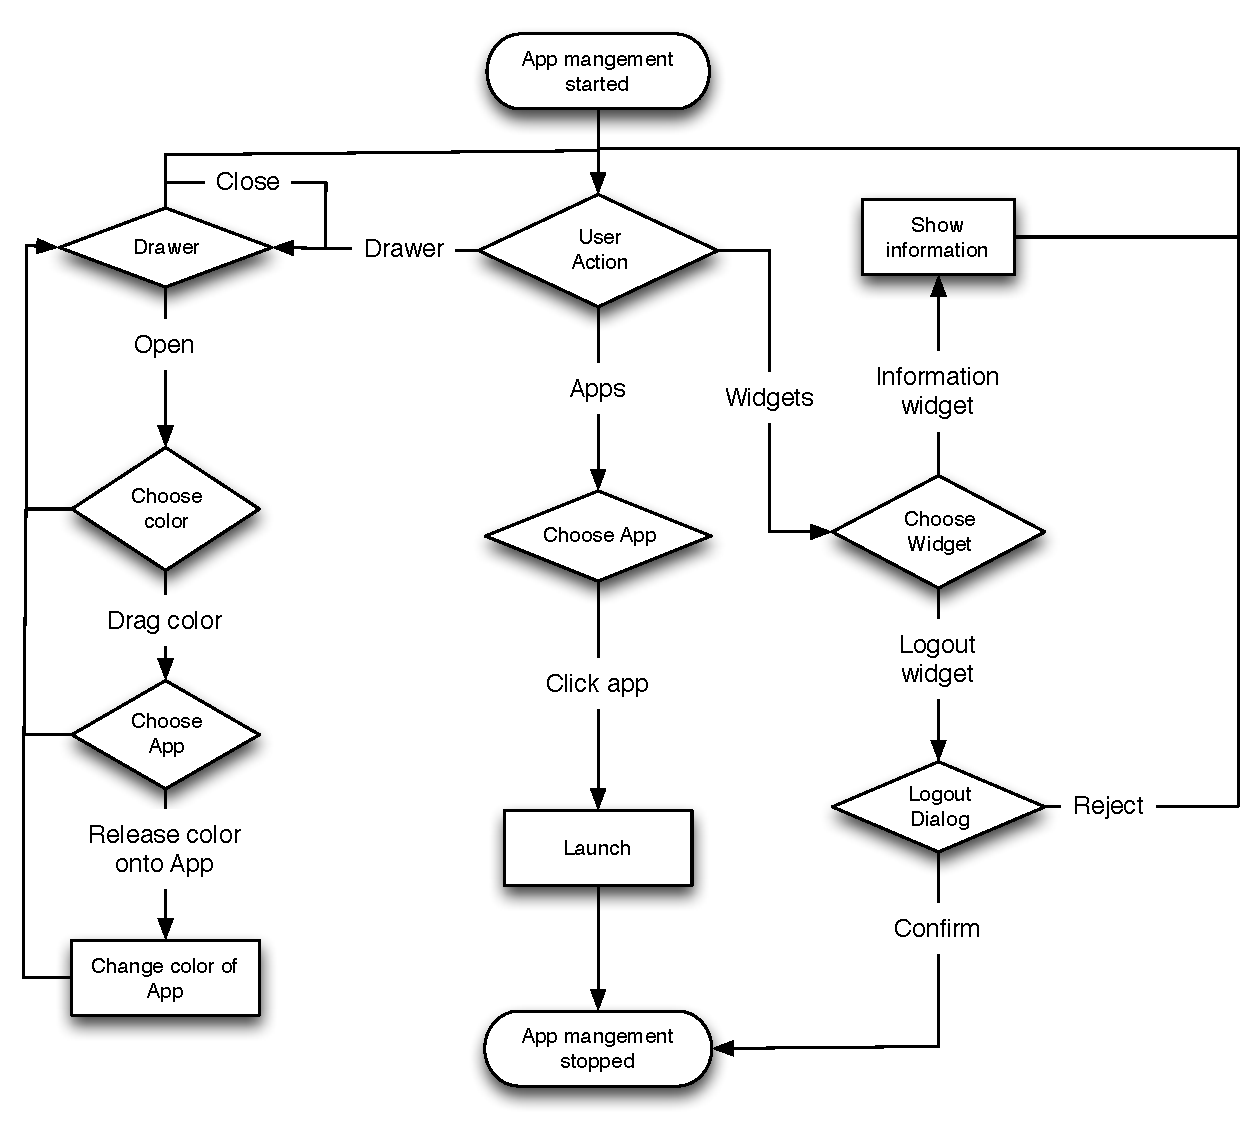
\includegraphics[width=1\textwidth]{gfx/appmanagement.pdf}
	\caption{Flowchart over the app management functionality}
	\label{fig:appmanagement_design}
\end{figure}

\autoref{fig:appmanagement_design} shows three branches of interactions and actions:

\begin{itemize}
	\item Change app settings
	\item Launch app
	\item Request information
\end{itemize}


\subsubsection{The drawer}
\label{sec:drawer}
The drawer was designed to hide functionallity when not needed in a convenient place. As seen in \autoref{fig:appmanagement_design} everything that have to do with changing app settings is placed in the drawer which the user have to open to get to it.
Another thing the drawer did was to make a place for the widgets.
The handle of the drawer was designed to have the same color as the inside of the drawer because it was important to make consistensy in the way that the user should feel when they saw the color of the handle the thought of the functionality inside of the drawer. It was also rounded to tell the user that this element was interactive.

\paragraph{Widgets}
\label{par:widgets}
Widgets in the \giraf[] system should help the user request information. As seen in \autoref{fig:appmanagement_design} the user can take the action to request information. If the user chooses an information the information will be selected and shown to the user.
The reason it was designed this way is that if all the information should be around the drawer handle it would probatly confuse the user more than it would help them.
All widgets is designed so they need to be unique, meaning that there can never be two of the same widgets. This was done for making widgets more consistent so the user always would get the same information from the same widget. All widgets is also designed with round corners to seem interactive see \autoref{design:button_design}.
The logout widget should be in the bottom of the drawer because it should not confuse the user while they are looking for information.

\paragraph{Color picker}
\label{par:colorpicker}
All colors in the color picker is rounded because they are an interactive element. They also have white sides so they not fall into one with the background. The color picker consists of ten predefined colors. The reason for predefined colors in the color picker is to make contrast. If developers of \giraf[] apps made their app icons mono-colored in white the contrast would always be sufficient. This should help that all users will always see the icon no matter what icon background color was chosen.